\documentclass[border=14pt]{standalone}
\usepackage{tikz}
\usetikzlibrary{arrows.meta,positioning,shapes.geometric,shapes.misc,calc}
% --- dark theme (matches the tool's slate-900 panels) ---
\definecolor{bg}{HTML}{0F172A}       % background
\definecolor{boxfill}{HTML}{1E293B}  % operators
\definecolor{methfill}{HTML}{334155} % nodes / methods
\definecolor{stroke}{HTML}{64748B}
\definecolor{txt}{HTML}{E2E8F0}
\definecolor{arrowc}{HTML}{94A3B8}
\pagecolor{bg}
\begin{document}
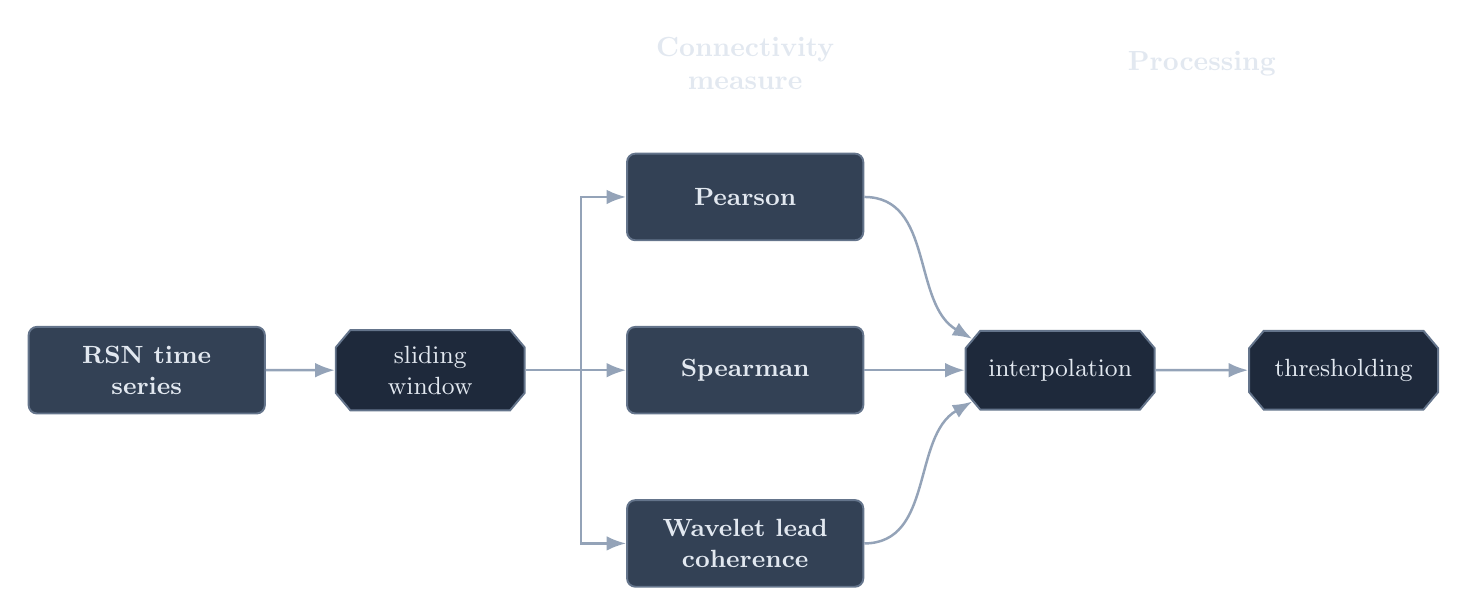
\begin{tikzpicture}[
  >=Latex,
  every node/.style={text=txt},
  proc/.style={rounded corners=3pt, draw=stroke, line width=0.7pt, fill=methfill,
     align=center, inner sep=5pt, minimum height=11mm, minimum width=30mm,
     font=\bfseries\small},
  meth/.style={proc},
  op/.style={chamfered rectangle, chamfered rectangle angle=40,
     draw=stroke, line width=0.7pt, fill=boxfill,
     align=center, inner sep=3pt, minimum height=10mm, minimum width=24mm, font=\small},
  hdr/.style={font=\bfseries, align=center, text=txt},
  arr/.style={->, line width=0.9pt, draw=arrowc},
  bus/.style={line width=0.9pt, draw=arrowc},
]
% --- columns ---
\def\xrsn{2.8}  \def\xsw{6.4}  \def\xm{10.4}
\def\xint{14.4}  \def\xthr{18.0}
% --- rsn ---
\node[proc] (rsn) at (\xrsn,0) {RSN time\\series};
% --- sliding window (before the correlations) ---
\node[op] (sw) at (\xsw,0) {sliding\\window};
% --- methods ---
\node[meth] (pear)  at (\xm, 2.2) {Pearson};
\node[meth] (spear) at (\xm, 0.0) {Spearman};
\node[meth] (wav)   at (\xm,-2.2) {Wavelet lead\\coherence};
% --- processing operators ---
\node[op] (int) at (\xint,0) {interpolation};
\node[op] (thr) at (\xthr,0) {thresholding};
% --- headers ---
\node[hdr] at (\xm,   3.9) {Connectivity\\measure};
\node[hdr] at ({(\xint+\xthr)/2}, 3.9) {Processing};
% --- arrows ---
\draw[arr] (rsn) -- (sw);
% branch sliding window -> methods
\coordinate (b) at ($(sw.east)+(0.7,0)$);
\draw[bus] (sw.east) -- (b);
\draw[arr] (b) |- (pear.west);
\draw[arr] (b) |- (spear.west);
\draw[arr] (b) |- (wav.west);
% methods merge -> interpolation
\draw[arr] (pear.east)  to[out=0,in=150] (int.north west);
\draw[arr] (spear.east) -- (int.west);
\draw[arr] (wav.east)   to[out=0,in=210] (int.south west);
% chain
\draw[arr] (int) -- (thr);
\end{tikzpicture}
\end{document}
